Question:\\
\emph{
    Web exercise:
- Recommend a DW DBMS for the Census Bureau.\\\\ The list is open, but examples
are PostgreSQL, CockroachDB, TiDB, SingleStore MemSQL and ClickHouse.\\ Your
recommendation should be based on five criteria. You are supposed to score
three vendors. Scoring should be based on data you collect from web sources.
See below hint:}\\

Kim-input: A list with 10 different criteria for (or features of) DW DBMS is presented in 
the lecture notes. \footnote{See document: 00 DBII-Part II-2025-AE, p.11} 

\begin{figure}[h] % "h" means "here"
    \centering
    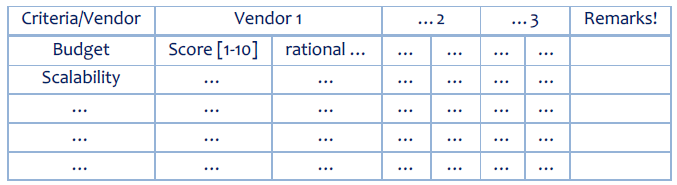
\includegraphics[width=0.5\textwidth]{Figures/Q7_QUESTION_table.PNG}
    \label{fig:my_image}
\end{figure}

\emph{[00:15:13] question number seven that's a web exercise and and i have talked about that
um in the beginning of the lectures so i recommend a data warehouse engine so a dbms engine for the
census office of course if you google you will um the term i mean what is the data warehouse engine used
for example by the swedish census office or finnish or us or german or etc they all are using by the way
and then you will get some uh case studies telling yeah those are using for example oracle technology
those are using pulse to grass and those are using teradata and yeah uh green plum and a lot of names
it's only uh some names that i have put here so so that the question here that i want to
yeah uh like test your ability to compare and recommend the technology so the name is not important so for
once again there is no model answer here to the name so for example if you ended up saying it's a tie db
and somebody else said no it's a single store and third student said it's a click house you all might
be right yeah as long as you have evaluated those options and put a criteria this is an exercise on
evaluation rather than an exercise on selection uh can we evaluate yeah what are the evaluation criteria
i put examples here like scalability and i talked about scalability in the course
or budget which one is cheaper uh yeah or which one is most expensive usually the cheapest gets the
highest points and the most expensive gets the lowest points when it comes to the budget criteria
which one is a scalable horizontal and vertical and we have talked about this and so forth so so you need
to collect the data um and compare}\\

\newpage Answers to Question 7:
\section{The Web Exercise}
This question requires a web exercise,therefore we have decided to add sections, one for each product. 

\subsection{Choice of criteria:}
The criteria we have chosen to evaluate the vendors and why are:
\begin{itemize}
    \item Scalability: This is an important criteria since:
    \begin{quotation}
        "Can we scale up, so this is important [...] the goverment is opening up it's database to the public for example.[...] so scalable means it can support more users and larger data volume"\cite[t.00:53:00]{l1video}".
    \end{quotation}
    \item Storage: Storage is an important criteria since
    the DBMS must efficiently handle large volumes of data, 
    ensuring optimal load performance and storage management to 
    accommodate growing datasets without architectural limitations \cite[p. 1239]{CourseLitt}.
    \item Cost: This is an important criteria since developing a DBMS is a costly endeavour, and the cost of the chosen DBMS can add or substract from this. \begin{quotation}
        "the cost can vary enormously from tens of thousands to millions of dollars due to
    the variety of technical solutions available." \cite[p. 1226]{CourseLitt}
    \end{quotation}
    \item Security: \begin{quote}
        "Security is critical to the data warehouse. To provide the strongest possible
security and to minimize administrative overhead, all security policies are enforced
within the data warehouse."\cite[p. 1309]{CourseLitt}
    \end{quote}
    \item Latency: This is an important criteria since \begin{quotation}
         "the DBMS must be able to handle large, complex queries for key business operations that must complete in reasonable time periods." \cite[p. 1239]{CourseLitt}
    \end{quotation} 
\end{itemize}
\begin{comment}
\begin{itemize}
    \item Scalability:
    \item Storage: 
    \item Cost:
    \item Security:
    \begin{itemize}
        \item Data Encryption:
        \item Access Control:
        \item Security Certificates:
    \end{itemize}
    \item Latency:
\end{itemize}   
\end{comment}
\subsection{Vendor 1 - ClickHouse:}
\begin{itemize}
    \item Scalability: ClickHouse allows for multiple nodes which eases horizontal scalability, 
    ClickHouse does not automatically shard, and re-sharding your dataset will require significant compute resources. \cite{clickhouseScaling}
    Given ClickHouse's provided example of a big data warehouse hardware specifications, vertical scaling seems to be well supported \cite{clickhouseScaling}.
    \item Storage: Clickhouse uses a column-oriented storage model, which is efficient for analytical queries \cite{clickhouseStorage}. ClickHouse is not inherently designed for in-memory usage \cite{clickhouseStorage}.
    In the benchmark ClickHouse scores the highest in terms of storage size reduction (See Storage Size under Appendix~\ref{sec:benchmarks}).
    \item Cost: ClickHouse is free to deploy and use, and is open-source \cite{clickhouseCost}.
    \item Security: 
    \begin{itemize}
        \item Data Encryption: Supports data encryption with AES 256 keys and Transparent Data Encryption (TDE) \cite{clickhouseSecurity}.
        \item Access Control: Supports Role-based access control and multi-factor authentication (MFA) \cite{clickhouseSecurity2}
        \item Security Certificates: ISO 27001 compliance, SOC 2 Type II compliance, GDPR and CCPA compliance, HIPAA compliance \cite{clickhouseSecurity2}
    \end{itemize}
    \item Latency: Clickhouse scores the highest in terms of latency (See Hot Run and Cold Run under Appendix~\ref{sec:benchmarks}).
\end{itemize}    
\subsection{Vendor 2 - SingleStore:}
\begin{itemize}
    \item Scalability: allows both vertical and horizontal scaling. Horizontal scaling through nodes \cite{singlestoreScaling}. SingleStore does automatically shard \cite{SinglestoreSharding}.
    \item Storage: Can be modified to have either column- or row-oriented storage \cite{singlestoreStorage}. SingleStore is designed for in-memory usage \cite{singlestoreStorage}.
    In the benchmark SingleStore scores worse than ClickHouse but far better than PostgreSQL in terms of storage size reduction (See Storage Size under Appendix~\ref{sec:benchmarks}).
    \item Cost: SingleStore is charged at individual rates (no publically available fixed fee) \cite{singleStoreCost}.
    \item Security: 
    \begin{itemize}
        \item Data Encryption: SingleStore automatically enforces AES 256-bit encryption \cite{singlestoreSecurity}.
        \item Access Control: SingleStore supports Row-Level Security (RLS) \cite{singlestoreSecurity2}.
        \item Security Certificates: SOC 2 Type 2, HIPAA, CCPA, GDPR \cite{singlestoreSecurity3}.
    \end{itemize}
    \item Latency: SingleStore scores worse than ClickHouse but far better than PostgreSQL in terms of latency (See Hot Run and Cold Run under Appendix~\ref{sec:benchmarks}).
\end{itemize} 
\subsection{Vendor 3 - PostgreSQL:}
\begin{itemize}
    \item Scalability: PostgreSQL can scale horizontally but it is difficult and convoluted to implement \cite{postgresqlHorScaling}.
    PostgreSQL is however known to be able to scale vertically rather well \cite{postgresqlVerScaling}.
    \item Storage: PostgreSQL is traditionally a row-oriented database management system (DBMS), but it supports columnar storage through extensions \cite{postgresqlStorage}.
    In the benchmark PostgreSQL scores the worst by a large margin in terms of storage size reduction (See Storage Size under Appendix~\ref{sec:benchmarks}).
    \item Cost: PostgreSQL is free to deploy and use, and is open-source \cite{postgresqlCost}.
    \item Security:
    \begin{itemize}
        \item Data Encryption: PostgreSQL supports Transparent Data Encryption (TDE) \cite{postgresqlSecurity} and, with the help of an extension, Column-Level Encryption with AES-256 \cite{postgresqlSecurity2}.
        \item Access Control: PostgreSQL supports Role-Based Access Control (RBAC) \cite{postgresqlSecurity3} and Row-Level Security (RLS) \cite{postgresqlSecurity4}.
        \item Security Certificates: None found.
    \end{itemize}
    \item Latency: PostgreSQL scores by far the worst in terms of latency (See Hot Run and Cold Run under Appendix~\ref{sec:benchmarks}).
\end{itemize} 
\section{The Comparison}
In this section we provide a comparison between vendors, therefore we have decided to add sections, one for each criterion. 

\subsection{Criteria 1 - Scalability:}
All three DBMS:s have good support for vertical scaling.
Both ClickHouse and SingleStore are designed to scale horizontally through sharding. ClickHouse does not automatically shard, and re-sharding your dataset will require significant compute resources \cite{clickhouseScaling}. SingleStore does automatically shard \cite{SinglestoreSharding}. PostgreSQL can scale horizontally but it is difficult and convoluted to implement \cite{postgresqlHorScaling}.
\\\\
As such, the three DBMS are ranked as follows, with the best first:

\begin{enumerate}
    \item SingleStore
    \item ClickHouse
    \item PostgreSQL
\end{enumerate}
\subsection{Criteria 2 - Storage:}
Both ClickHouse and SingleStore can use column-oriented storage, which is effecient for OLAP systems as formerly mentioned. PostgreSQL does not natively support columnar storage.
ClickHouse is not inherently designed for in-memory usage \cite{clickhouseStorage}, while SingleStore is designed for in-memory usage \cite{singlestoreStorage}.
As per optimizing storage size, ClickHouse scores the highest, SingleStore scores second, and PostgreSQL scores the lowest by a  far margin.
\\
Here which rankest the highest is not very clear, given that ClickHouse is not designed for in-memory usage, which is a disadvantage in terms of efficiency. However, ClickHouse scores the highest in terms of storage size reduction.
Since the writers of this report are not experts in the field and given the aforementioned uncertainty, we will rank ClickHouse and SingleStore the highest for the sake of fairness. 
\\\\
As such, the three DBMS are ranked as follows, with the best first:

\begin{enumerate}
    \item SingleStore \& ClickHouse
    \item PostgreSQL
\end{enumerate}
\subsection{Criteria 3 - Cost:}
Both PostgreSQL and ClickHouse are free to deploy and use, and are open-source \cite{clickhouseCost} \cite{postgresqlCost}. SingleStore is charged at individual rates \cite{singleStoreCost}.
\\\\
As such, the three DBMS are ranked as follows, with the best first:

\begin{enumerate}
    \item PostgreSQL \& ClickHouse
    \item SingleStore
\end{enumerate}
\subsection{Criteria 4 - Security:}
As per data encryption, all three DBMS:s support AES 256-bit encryption.\\
As per access control, Both SingleStore and PostgreSQL allow for Row-Level Security (RLS), while ClickHouse does not.
ClickHouse is the only DBMS found to support multi-factor authentication.\\
As per security certifications, postgreSQL does not seem to have any, whereas both SingleStore and ClickHouse have several.
However, ClickHouse is the only one who has a \textit{ISO 27001} certification. The \textit{ISO 27001} \textit{"certification demonstrates that an organisation has defined and put in place best-practice information security processes. "}\cite{ISO27001}.
\\\\
As such, the three DBMS are ranked as follows, with the best first:

\begin{enumerate}
    \item ClickHouse
    \item SingleStore
    \item PostgreSQL
\end{enumerate}

\subsection{Criteria 5 - Latency:}
As seen in the benchmark Appendix~\ref{sec:benchmarks}, ClickHouse scores the best in terms of latency, SingleStore scores second, and PostgreSQL scores the worst by a large margin.
\\\\
As such, the three DBMS are ranked as follows, with the best first:

\begin{enumerate}
    \item ClickHouse
    \item SingleStore
    \item PostgreSQL
\end{enumerate}

\section{Conclusion}
In favor of offering a quick overview of the ranking of the different criterias for each DBMS, a table is provided below with scoring per criteria for each DBMS. 
If the DBMS came first in a criteria, it was awarded 3 points, if it came second it was awarded 2 points, and if it came last it was awarded 1 point.

\begin{table}[h]
    \centering
    \begin{tabular}{|c|c|c|c|c|c|c|}
    \hline
    \textbf{DBMS} & \textbf{Scalability} & \textbf{Storage} & \textbf{Cost} & \textbf{Security} & \textbf{Latency} & \textbf{Total} \\ \hline
    ClickHouse & 2 & 3 & 3 & 3 & 3 & 14 \\ \hline
    SingleStore & 3 & 3 & 1 & 2 & 2 & 11 \\ \hline
    PostgreSQL & 1 & 1 & 3 & 1 & 1 & 7 \\ \hline
    \end{tabular}
    \caption{Scoring per criteria for each DBMS}
    \label{tab:my-table}
\end{table}